\documentclass{cmspaper}
\def\RCS$#1: #2 ${\expandafter\def\csname RCS#1\endcsname{#2}}
\RCS$Revision: 1.2 $
\RCS$Date: 2004/05/27 12:46:29 $

\usepackage{graphicx}

\begin{document}
\begin{titlepage}
  \whitepaper
  \date{Revision \RCSRevision, \RCSDate}
  \title{CMS Data Handling: TMDB Schema and Database Interactions}

  \begin{Authlist}
    Tim~Barrass, Simon~Metson\Instfoot{bristol}{University of Bristol, Bristol, UK}
    Lassi~A.~Tuura\Instfoot{neu}{Northeastern University, Boston, USA}
  \end{Authlist}

  \begin{abstract}
    This white paper describes the database schema for the CMS data
    handling system. I also defines the expected set of agent-TMDB
    interactions (effectively outlining the functionality of each
    agent).
  \end{abstract}

  \note{DRAFT version}
\end{titlepage}

\setcounter{page}{2}

\section{Transfer Management Database}

\begin{figure}[tbp]
\centering
  \includegraphics[width=15cm]{tmdb-schema.eps}
  \caption{Entities and relations in the TMDB V2.  Basic SQL
    to create is detailed in the appendix.}
   \label{fig:schema}
\end{figure}

\begin{description}
  \item [\texttt{t\_Nodes}]\mbox{}

    Table is just a reference against which node names are constrained
    unique.  \verb|host_string| is a small string that can be used to
    identify SURLs of files that reside on that node.

  \item [\texttt{t\_Files\_for\_transfer}]\mbox{}

    Agents make an entry in this table when they make data available
    for distribution.

    [Note that it's possible to add a file catalogue table
    here---whether it will be performant is a different issue.
    Problem is that LCG tools expect a webservice front end to the
    FC... is this really a problem if we use
    SRM+gridFTP+catalogue(POOL?) registration?]

  \item [\texttt{t\_Destinations}]\mbox{}

    The configuration agent finds new files for distribution and makes
    destination entries here.  A GUID may appear multiple times (if it
    is directed toward multiple destinations).

    The configuration agent also needs to make the first advertisement
    of the file.  Using the source and destination nodes, uses the
    routing table to determine the first gateway and makes the
    relevant entry in \texttt{t\_Current\_state}.

  \item [\texttt{t\_Current\_state}]\mbox{}

    The configuration agent and transfer agents post state in this
    table. There should be an entry here for each replica in of a
    given GUID in distribution.

    The states recorded in current state can be a lot simpler than in
    v1: {\em in transfer}, {\em available}, {\em safe}, {\em clean}.

    An important difference between this state table and the previous
    version is that no entries should be replaced---entries should just
    be added, maintaining a log of the progress of GUIDs through
    states at each node.

  \item [\texttt{t\_Config\_messages}]\mbox{}

    For this version we only need very simple steering: {\em resume},
    {\em suspend}, {\em stop}.

    A global client might post {\em <t1 : SUSPEND : A : false>} to suspend
    node A.  A's agent manager would need to find that message, suspend
    agent at A and mark the message as handled = true.

    By marking entries handled rather than just deleting them we
    retain a log of global system changes.

  \item [\texttt{t\_Agents}]\mbox{}

    Provides a reference against which agent names can be checked.

  \item [\texttt{t\_Lookup}]\mbox{}

    Very similar to original \texttt{agentstate}:
    {\em <Node name : agent name : state : last contact>}

    This allows for more sophisticated states than up or down... we
    could just have agent as a unique key here, and lose the agent
    table.  However, we want to indicate the state of nodes and of
    agents here, so null entries under agent are possible.

  \item [\texttt{t\_File\_allocation\_config}]\mbox{}

    Stores global stream->destination configuration.  This used to be
    written into a text file read by the configuration agent.

  \item [\texttt{t\_Replica\_metadata}]\mbox{}

    Allows storage of replica metadata (file size, checksum, specific
    states, etc) coupled to GUIDs.  In DC04 we found that we needed to
    add new meta data to GUIDs as new functionality appeared in the
    system (``filegroup'' for real time analysis).  This meant tying
    down the DB while adding fields to tables with a large number of
    entries.  By having a separate table for this meta data we can add
    meta data as necessary.

    [Is it worth placing some limit/schema on the meta data?  Thinking
    it through it could be used for some quite creative purposes.]

  \item [\texttt{t\_Routing}]\mbox{}

    A global routing table, should be partitioned on from (basically
    creating the same set of tables as a distributed system of
    routers).  The routing algorithm is described below.
\end{description}





\section{Requirement of sources of data and agents}
\subsection{Typical agent-transfer management database communication}
The following discussion doesn't include interactions with the logging
database, or processes such as agent state publishing and other system
maintenance tasks.  Instead, it is intended to give a feel for the flow
of data through the system.

\subsection{Data sources}
To make data available for distribution:
{\small\begin{verbatim}
  insert into t_Files_for_transfer
    values (guid, source_node, time, checksum, 0);
\end{verbatim}}

The data sources will also need to add the first metadata to the system.

\subsection{Configuration agent}

The configuration agent will scan \texttt{t\_Files\_for\_transfer}
looking for unallocated files (allocated = 0).  Using configuration
information it will allocate files to specific nodes by making entries
in \texttt{t\_Destinations} and \texttt{t\_Current\_state}:

First find new files for transfer

{\small\begin{verbatim}
  select guid, source_node
  from t_Files_for_transfer
  where allocated = 0;
\end{verbatim}}

Determine file allocation.  First it needs to query the POOL meta data
to determine the file stream, then it needs to look up the stream
(here it's done dynamically, but it could rebuild an internal table
every loop...)

{\small\begin{verbatim}
  select destination from t_File_allocation_config
  where stream = ``the_stream'';
\end{verbatim}}

For each destination, make entries in \texttt{t\_Destinations}.

{\small\begin{verbatim}
  insert into t_Destination
    values (guid, destination);
\end{verbatim}}

Now lookup the gateway for each destination from the source node

{\small\begin{verbatim}
  select * from
    (select gateway, hops
     from t_Routing
     where from = ``source_node''
       and to = ``destination''
     order by hops asc)
  where rownum = 1;
 \end{verbatim}}

For each gateway, make an entry advertising the file in \texttt{t\_Current\_state}:

{\small\begin{verbatim}
  insert into t_Current_state
    values (guid, gateway, ``available'',
            currenttime, source_node);
\end{verbatim}}

It also needs to mark the guid as allocated...

\subsection{Transfer agents}

Transfer agents search \texttt{t\_Current\_state} for files advertised
for them.  They copy those files, work out where to send them next (ie
function basically as a router) and advertise them accordingly.

This example is for a transfer agent at a node named ``Foo''.

First, search for new files:

{\small\begin{verbatim}
  select guid, is_at_node
  from t_Current_state
  where is_for_node = 'Foo'
  and state = 'available';
\end{verbatim}}

which might produce a set of guids {guid1, guid2, guid3 ...} currently at nodes {Bar1, Bar2, Bar3 ...}. The start of transfer of each guid should be marked by posting state- e.g. for guid1 at Bar1 to Foo

{\small\begin{verbatim}
  insert into t_Current_state
    values (guid1, 'Foo', 'in transfer',
            currenttime, 'Bar1');
\end{verbatim}}

Transfer the file, then mark as complete by posting state

{\small\begin{verbatim}
  insert into t_Current_state
    values (guid, 'Foo', `on buffer',
            currenttime, 'Bar1');
\end{verbatim}}

The set of desinations for each guid needs to be determined

{\small\begin{verbatim}
  select destination
  from t_Destinations
  where guid = guid1;
\end{verbatim}}

which might, for guid1, produce the set of destination nodes {Dest1, Dest2, ...}. For each destination the appropriate gateway (or next hop in the chain) needs to be determined, e.g. for guid1 going to Dest1

{\small\begin{verbatim}
  select * from
    (select gateway, hops
     from t_Routing
     where from = 'Foo'
       and to = 'Dest1'
     order by hops asc)
  where rownum = 1;
\end{verbatim}}

Which might retutn the gateway Gate1. Finally advertise the newly available file

{\small\begin{verbatim}
  insert into t_Current_state
    values (guid, 'Gate1', ``available'',
            currenttime, 'Foo');
\end{verbatim}}

[ To some extent I've tried to parcel this up so some element of failure recovery can be undertaken. e.g. if there are entries saying "on buffer" but not "available", then obviously the next hop for guids "in buffer" needs to be determined and them advertised as available appropriately. ]

\subsection{Mass storage agents}
These are an extension of the transfer agent---when they have made a
file safe in mass storage they should advertise it as ``safe''.

\subsection{Buffer cleaning agents}

These agents should operate at each node. They should examine the
state of each file at all sites (long inefficient query?). They need
to decide whether it is safe to delete the file based on some
criteria---a suitable criteria might be

``If the file is marked \`{O}safe\'{O} at two or more nodes, then it can be
deleted from this buffer.''

\section{SQL for the schema}

{\small \begin{verbatim}
CREATE TABLE t_Routing (
    from varchar NOT NULL,
    to varchar NOT NULL,
    gateway varchar NOT NULL,
    timestamp int NOT NULL,
    hops int NOT NULL,
    PRIMARY KEY(from));

CREATE TABLE t_Files_for_transfer (
    guid char[36] UNIQUE NOT NULL,
    source_node varchar NOT NULL,
    allocated char[1] NOT NULL,
    PRIMARY KEY(guid));

CREATE TABLE t_Nodes (
    node_name varchar UNIQUE NOT NULL,
    host_string varchar NOT NULL,
    PRIMARY KEY(node_name),
    FOREIGN KEY(node_name) REFERENCES t_Files_for_transfer (source_node),
    FOREIGN KEY(node_name) REFERENCES t_Routing (from),
    FOREIGN KEY(node_name) REFERENCES t_Routing (to),
    FOREIGN KEY(node_name) REFERENCES t_Routing (gateway));

CREATE TABLE t_Destinations (
    guid char[36] UNIQUE NOT NULL,
    destination_node varchar NOT NULL,
    PRIMARY KEY(guid),
    FOREIGN KEY(guid) REFERENCES t_Files_for_transfer (guid),
    FOREIGN KEY(destination_node) REFERENCES t_Nodes (node_name));

CREATE TABLE t_Current_state (
    guid char[36] UNIQUE NOT NULL,
    is_for_node varchar NOT NULL,
    state char[1] NOT NULL,
    timestamp int NOT NULL,
    is�t_node varchar NOT NULL,
    PRIMARY KEY(guid),
    FOREIGN KEY(guid) REFERENCES t_Files_for_transfer (guid),
    FOREIGN KEY(is_for_node) REFERENCES t_Nodes (node_name));

CREATE TABLE t_Lookup (
    node varchar NOT NULL,
    agent varchar,
    state char[1] NOT NULL,
    last_contact int NOT NULL,
    FOREIGN KEY(node) REFERENCES t_Nodes (node_name),
    FOREIGN KEY(agent) REFERENCES t_Agents (name));

CREATE TABLE t_Config_messages (
    node varchar NOT NULL,
    message varchar NOT NULL,
    timestamp int NOT NULL,
    handled char[1] NOT NULL,
    FOREIGN KEY(node) REFERENCES t_Nodes (node_name));

CREATE TABLE t_File_allocation_config (
    stream varchar NOT NULL,
    destination varchar NOT NULL,
    FOREIGN KEY(destination) REFERENCES t_Nodes (node_name));

CREATE TABLE t_Agents (
    name varchar UNIQUE NOT NULL,
    PRIMARY KEY(name));

CREATE TABLE t_Replica_metadata (
    guid char[36] UNIQUE NOT NULL,
    key varchar NOT NULL,
    value varchar,
    PRIMARY KEY(guid),
    FOREIGN KEY(guid) REFERENCES t_Files_for_transfer (guid));
\end{verbatim}}

\end{document}
